\section{Model analityczny}
Celem niniejszego rozdziału jest zdefiniowanie, jak wyglądać będzie architektura tworzonego systemu. Aby to osiągnąć, w~rozdziale załączone zostały diagramy wykonane zgodnie ze~standardem UML, które stanowią wizualną reprezentację architektury systemu oraz pozwalają na~łatwiejszą analizę stanu projektu.

\subsection{Diagram klas}
Przedstawiony poniżej diagram klas reprezentuje wszystkie wykorzystywane przez Zleceniodawcę elementy składające się na cały system. Diagram ten jest kluczowy przede wszystkim dla deweloperów oraz innych osób zajmujących się bezpośrednio wytwarzaniem oprogramowania, tym niemniej powinien zostać zatwierdzony także przez przedstawicieli Zleceniodawcy -- diagram klas jest bowiem punktem łączącym -- z~jednej strony wyobrażenie klienta o~podziale funkcjonalności, a~z~drugiej decyzje projektowe podjęte przez zespół zajmujący się implementacją.\\

\begin{figure}[H]
  \centering
  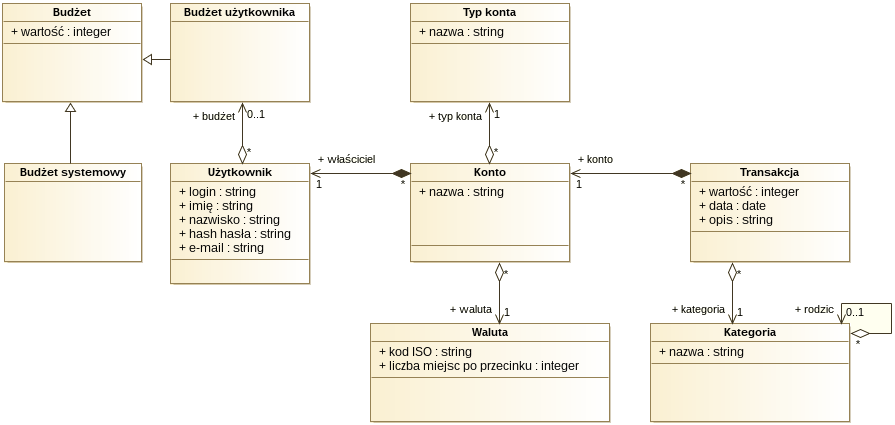
\includegraphics[width=\textwidth]{images/class-diagram.png}
  \caption{Diagram klas systemu.}
\end{figure}

Diagram klas obrazuje zależności (agregacje, kompozycje, relacje dziedziczenia) pomiędzy poszczególnymi klasami na~tyle szczegółowo, by~osoby nieposiadające wykształcenia informatycznego i~nieznające metod programowania obiektowego mogły zrozumieć zasadę podziału bez szczegółowych wyjaśnień. Wszystkie atrybuty czy operacje ważne z~punktu widzenia Zleceniodawcy, które mogą mieć wpływ na~ocenę projektu zostały umieszczone na~diagramie.
